\documentclass{article}
\usepackage[margin=2cm]{geometry}
\usepackage[latin1]{inputenc}
\usepackage{todo}
\usepackage{url}
\usepackage{caption}
\usepackage{subcaption}
\usepackage{graphicx}
\usepackage{listings}
\usepackage{color}
\usepackage{textcomp}

\definecolor{aliceblue}{rgb}{0.94, 0.97, 1.0}
\definecolor{almond}{rgb}{0.94, 0.87, 0.8}
\definecolor{asparagus}{rgb}{0.53, 0.66, 0.42}
\definecolor{gainsboro}{rgb}{0.86, 0.86, 0.86}
\definecolor{gray(x11gray)}{rgb}{0.75, 0.75, 0.75}

\lstset{frame=tb,
  aboveskip=3mm,
  belowskip=3mm,
  showstringspaces=false,
  columns=flexible,
  basicstyle={\small\ttfamily},
  numbers=none,
  breaklines=true,
  breakatwhitespace=true,
  tabsize=4,
  language=C
}

\title{Fractal Drums}
\author{Knut Andre G. Prestsveen}
\begin{document}
\maketitle




\section{Abstract}
A numerical study of vibrations of fractal shaped drums. The 10 lowest vibration eigenmodes for a drum with a   fractal shaped boundary were computed using finite diferences, and the scaling of the integrated density of states were compared with the Weyl-conjecture and results for drums with smooth boundary.

\section{Introduction}
For any drum, it's size is related to the pitch of the sound it makes, and the larger the area, the lower the pitch. The question in mind for this study, is if the shape of the drum also affects the tone so that information about the drum's shape can be inferred from the tone, and this study spesifically studied drums shaped like quadratic Koch fractals.

The study was carried out numerically, and program code for generating the fractal and a system lattice, representing the drums boundary and skin respectively, were written. The eigenmodes of the drums vibration were then computed with finite differences, and to see if the Weyl-conjecture could could be used to infer information about the fractal boundary, the integrated density of states of the fractal drum were compared to that of a drum with smooth boundary and same area.

\section{Theory}\label{theory}
\subsection{The Weyl-conjecture}
The shape of the drum cannot be completely inferred from it's sound alone, but some information can be extracted. Firstly the area of the drum $A$ can be found from

\begin{equation}
    \label{area}
    A = 4*\pi ...,
\end{equation}
where $N(\omega)$ is the integrated density of states (IDOS), i.e. the number of eigenfrequencies smaller than the frequency $\omega$. Also Hermann Weyl conjectured that the second term in the asymptotic of $N(\omega)$ gives the length of the drums perimeter $L$, so that

\begin{equation}
    \label{weyl-conjecture}
    N(\omega) = \frac{A}{4*\pi}...
\end{equation}
in the limit of large $\omega$. Equation \ref{weyl-conjecture} is the Weyl-conjecture for the IDOS, and is proven correct under the assumption of a smooth boundary. This study tries to see what happens when the boundary is fractal.

\subsection{Quadratic Koch Fractal}\label{theory-koch}
The quadratic koch fractal is recursively generated by starting out with a square, dividing each of the sides into four equal pieces, and displace the two middle pieces one side length, one of them up the other down. This process is repeated recursively until reached desired recursion depth. The process is illustrated in \ref{generate-koch}.

\begin{figure}
    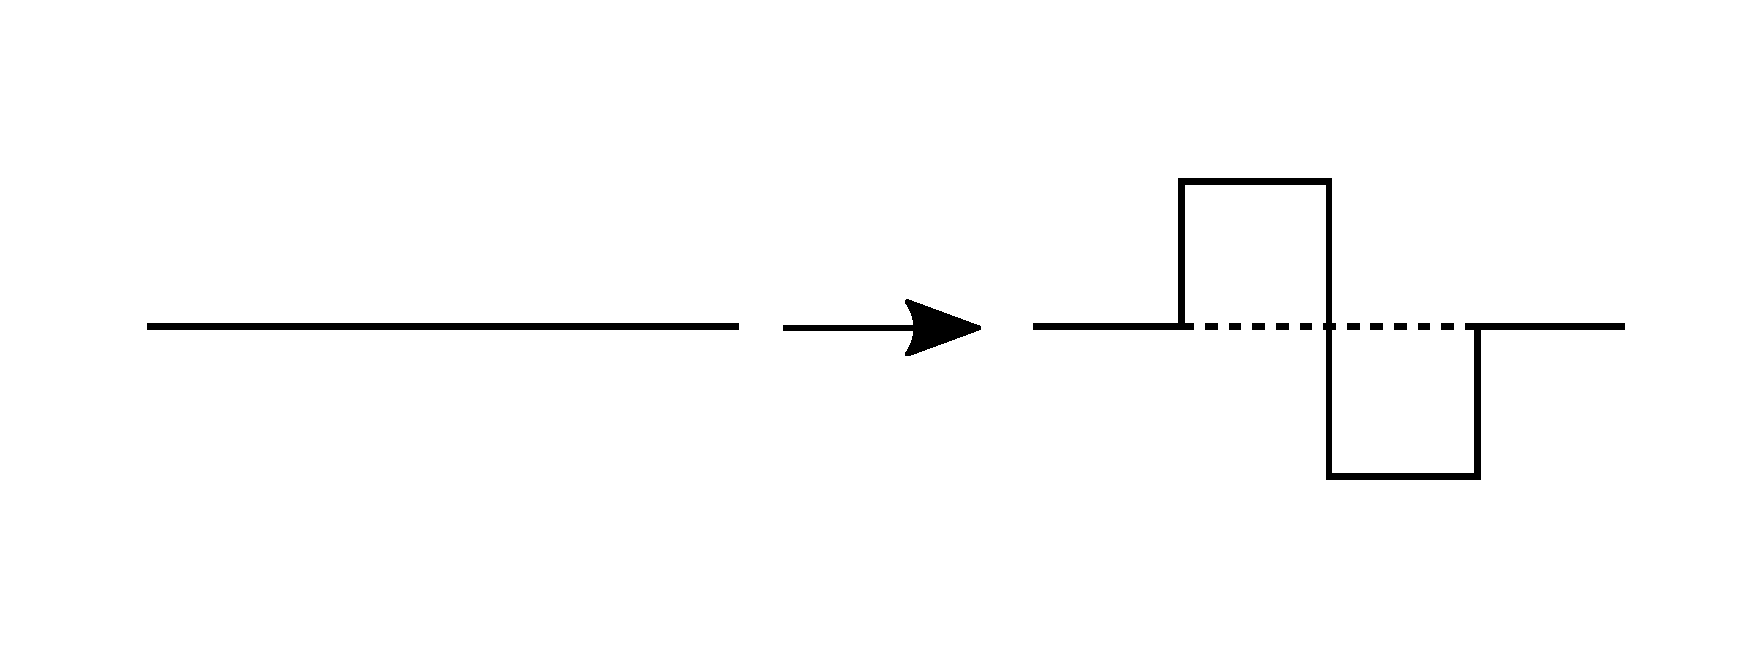
\includegraphics[width=\linewidth, trim={0 3cm 0 3cm}]{../figs/koch_frac_step.pdf}
    \caption{Koch fractal}
    \label{generate-koch}
\end{figure}

\subsection{The Helmholtz equation - Finite Difference Approximation}
The displacement of the drum's surface $u(r, t)$ is given by the wave equation \ref{wave-equation}, with the boundary conditions $u = 0$ on the boundary $\partial \Omega$. Performing the Fourier transform of the wave equation \ref{wave-equation} results in the Helmholtz equation \ref{helmholtz-equation}, and turns the problem into an eigenvalue problem.

\begin{equation}
    waveeq \\
\end{equation}

\begin{equation}
    HHeq \\
\end{equation}

The eigen values, and vectors of equation \ref{helmholtz-equation} were calculated using finite differences, with both the stantard five-point stensil and the nine-point stensil approximation to the laplacian operator. The discretization of equation \ref{helmholtz-equation} becomes

\begin{equation}
    five point
\end{equation}

and

\begin{equation}
    nine point
\end{equation}

for the five point and nine point approximations respectively.

\section{Code}
The program code is written in the julia language, the setup of the system is split into several files, which are all included in \colorbox{gainsboro}{\lstinline{setup.jl}}. The main script is \colorbox{gainsboro}{\lstinline{main.jl}}, which includes \colorbox{gainsboro}{\lstinline{setup.jl}} and solves the eigenvalue problem using the \colorbox{gainsboro}{\lstinline{eigs}} routine for sparse matrices from the ARPACK library.\\

\subsection{Fractal creation}\label{code:fractal}
The generation of the fractal is just a straight forward implementation of the recursive method described in \ref{theory-koch}. The code was split into three functions: firstly there is \colorbox{gainsboro}{\lstinline{generate_side}} which takes the start and end point of a side and returns the "transformed" side and \colorbox{gainsboro}{\lstinline{generate_corners}} which calls \colorbox{gainsboro}{\lstinline{generate_side}} for every side in the current fractal shape and for every level recursively, returning the alle the positions of the fractals corners.
Finally there is \colorbox{gainsboro}{\lstinline{fill_edges}} which places points on the sides between the corners, according to the specified grid constant.\\

\subsection{Determation of inside points}\label{code:determine-inside}
The determination of which points are inside is done with a breadth first like search, starting in the middle point which is known to be inside the fractal. Another method which was implemented starts in a point, scans towards the edge in one direction and uses the orientation of the curve to determin if the point was inside or not. The latter requieres that the fractals points are ordered correctly, was considerably slower, and while it could have been sped up considerably by determining every point along each scan in one go, this was not done
since the former method seemed more elegant. The lattice is first initialized with every element being \colorbox{gainsboro}{\lstinline{OUTSIDE}}, and the breadth search code is shown in listing \ref{lst:lattice-bfs}.\\

\begin{lstlisting}[label=lst:lattice-bfs]
    # --snip--    

    points = [left, right, down, up] 
    println("begin search")
    for point in points
        x, y = point
        if lattice[x, y] == OUTSIDE
            # New INSIDE point
            lattice[x, y] = INSIDE

            # Add nearest neighbours to points
            for nn in (-1, 1)
                    push!(points, (x + nn, y)) 
                    push!(points, (x, y + nn))
            end
        else
            continue
        end
    end 

    # --snip--    
\end{lstlisting}

\subsection{Datastructures}
The drum's surface is represented by a lattice, which in the code is a 2D array containing the enum type \colorbox{gainsboro}{\lstinline{Location}}, which can take the values \colorbox{gainsboro}{\lstinline{INSIDE}}, \colorbox{gainsboro}{\lstinline{OUTSIDE}} and \colorbox{gainsboro}{\lstinline{BORDER}}. Each points \colorbox{gainsboro}{\lstinline{Location}} value is determined by the process described in section \ref{code:determine-inside}, and the positions of the
points on the lattice are corresponding to the \colorbox{gainsboro}{\lstinline{CartesianIndices}} of the array.

For the alternative method of lattice creation, a slightly different representation was used. The lattice was then an array of the custom type \colorbox{gainsboro}{\lstinline{Point}}, which contains the membervariables \colorbox{gainsboro}{\lstinline{x::Int}}, \colorbox{gainsboro}{\lstinline{y::Int}} and \colorbox{gainsboro}{\lstinline{location::Location}}. The definitions of \colorbox{gainsboro}{\lstinline{Point}} and \colorbox{gainsboro}{\lstinline{Location}}
is shown in listing \ref{lst:datastructures}.\\

\begin{lstlisting}[label=lst:datastructures]
@enum Location INSIDE OUTSIDE BORDER


struct Point
    x::Int
    y::Int
    location::Location
end
\end{lstlisting}


\noindent
\textbf{Creation of laplacian matrix}\\
The negative laplacian matrix construction is also quite straight forward. It constructs the matrix row by row by looping through every lattice point inside the fractal, setting the diagonal elements to $4$ and the nearest neighbour elements to $-1$ if the neighbour also is an inside point. The definition of the function setting up the five point matrix is shown in listing \ref{code:five-point}, and the nine point version is completely analogous.\\

\begin{lstlisting}[label=code:five-point]
function five_point_laplacian(N, lattice, points_inside)
    println("Making laplacian matrix")
    lap_matrix = spzeros(N, N)
    for (idx, p) in enumerate(points_inside)
        x, y = p 
        lap_matrix[idx, idx] = 4 
        for nn in (-1, 1)
            if lattice[x+nn, y] == INSIDE
                nn_idx = findfirst(p -> p== (x+nn, y), points_inside)
                lap_matrix[idx, nn_idx] = -1
            end
            if lattice[x, y+nn] == INSIDE
                nn_idx = findfirst(p -> p== (x, y+nn), points_inside)
                lap_matrix[idx, nn_idx] = -1
            end
        end
    end 
    return lap_matrix
end
\end{lstlisting}

\section{Results}
Cool plots, and hopefully something clever about IDOS.

\begin{figure}
    \begin{subfigure}{0.5\textwidth}
        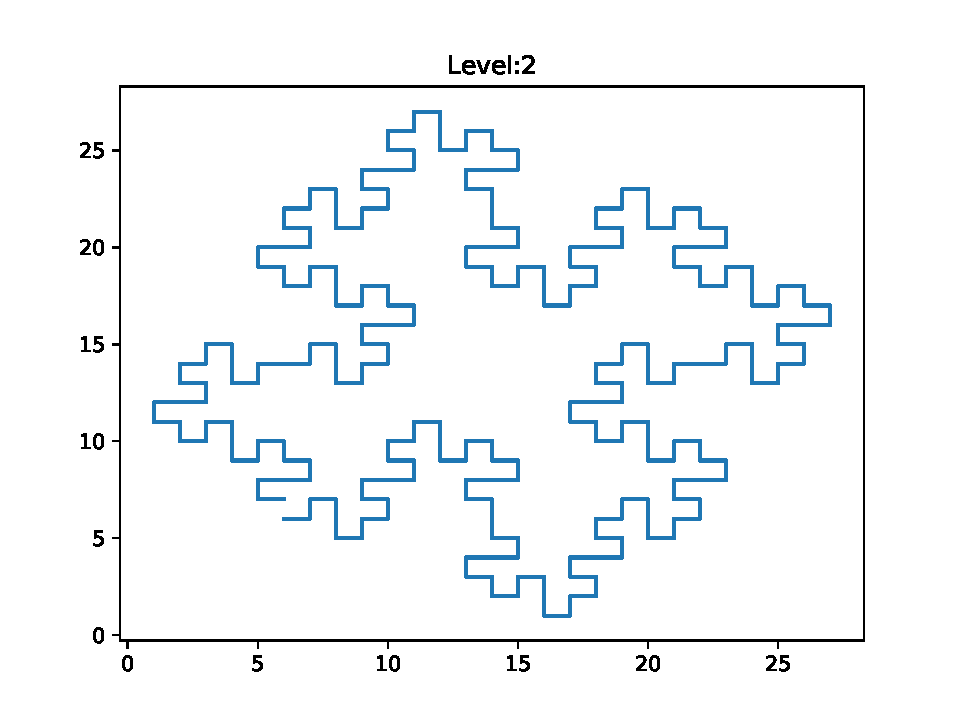
\includegraphics[width=\linewidth]{../figs/quad_koch_level2.pdf}
    \end{subfigure}
    \begin{subfigure}{0.5\textwidth}
        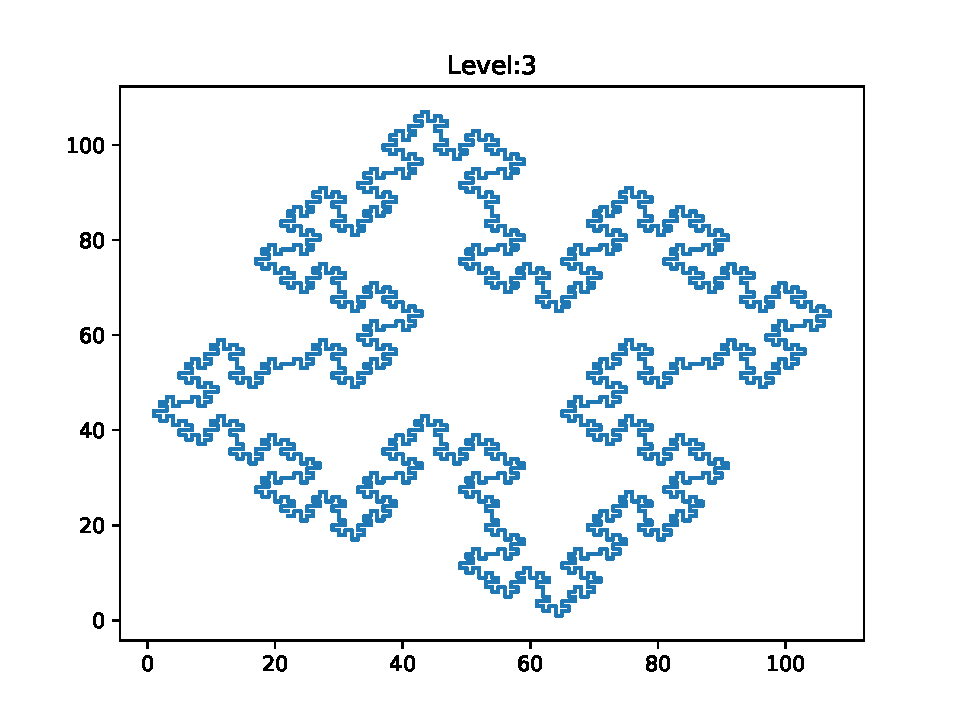
\includegraphics[width=\linewidth]{../figs/quad_koch_level3.pdf}
    \end{subfigure}
    \caption{Quadratic koch fractals of recursion depth 2 and 3, generated by the code described in \ref{code:fractal}}
\end{figure}

\subsection{Determin inside comparison}
Compare runtimes I guess

\subsection{Solutions to EV}
Table of eigenvalues (at least 10), ref to plots

\subsection{Largest value of L, memory}
L = 4, refer to possible suggestions in later section

\subsection{IDOS}

\subsection{Compare 9p to 5p stensil}
Compare some numbers, ev. runtimes



\newpage
\begin{figure}
    \begin{subfigure}{0.3\textwidth}
        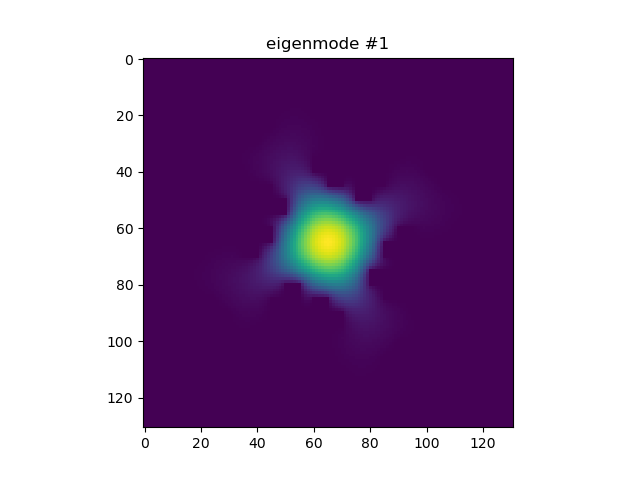
\includegraphics[width=\linewidth]{../figs/eigenmode_2d1.png}
    \end{subfigure}
    \begin{subfigure}{0.3\textwidth}
        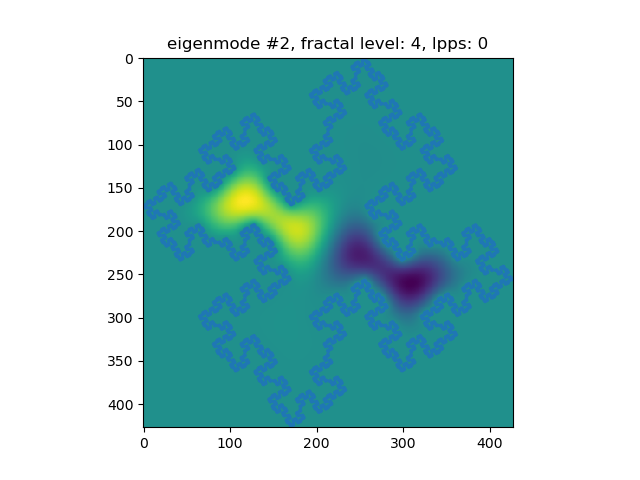
\includegraphics[width=\linewidth]{../figs/eigenmode_2d2.png}
    \end{subfigure}
    \begin{subfigure}{0.3\textwidth}
        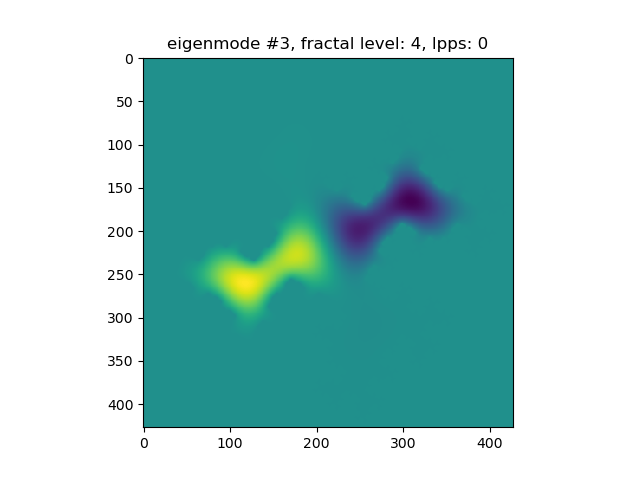
\includegraphics[width=\linewidth]{../figs/eigenmode_2d3.png}
    \end{subfigure}
    \begin{subfigure}{0.3\textwidth}
        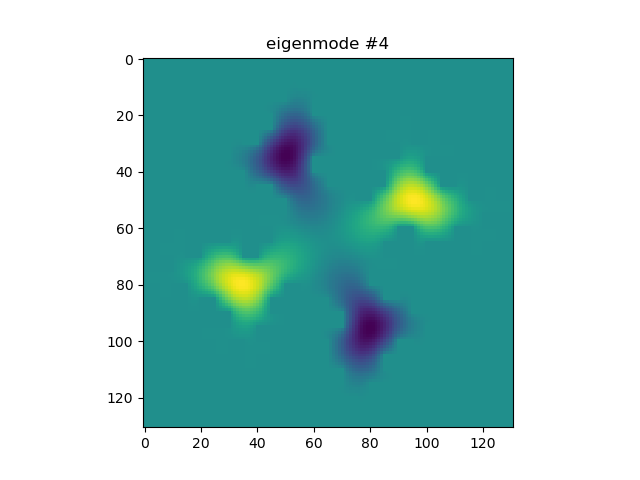
\includegraphics[width=\linewidth]{../figs/eigenmode_2d4.png}
    \end{subfigure}
    \begin{subfigure}{0.3\textwidth}
        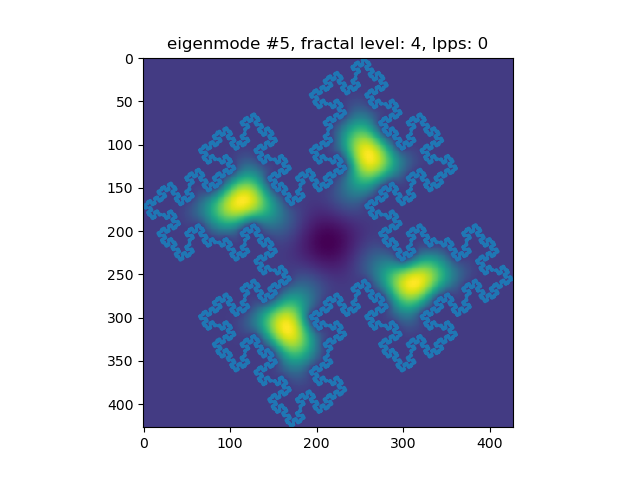
\includegraphics[width=\linewidth]{../figs/eigenmode_2d5.png}
    \end{subfigure}
    \begin{subfigure}{0.3\textwidth}
        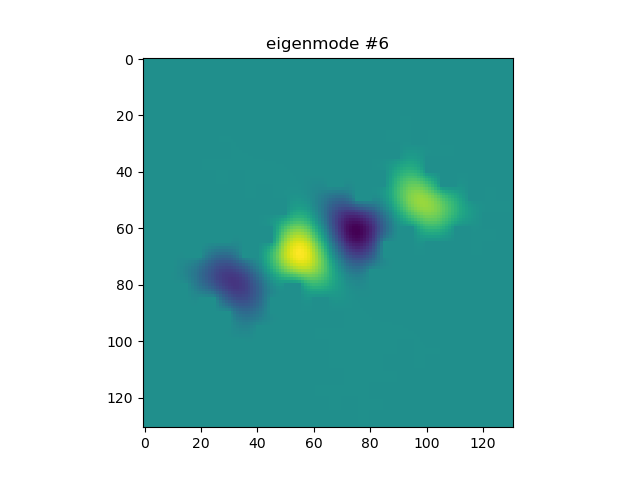
\includegraphics[width=\linewidth]{../figs/eigenmode_2d6.png}
    \end{subfigure}
    \begin{subfigure}{0.3\textwidth}
        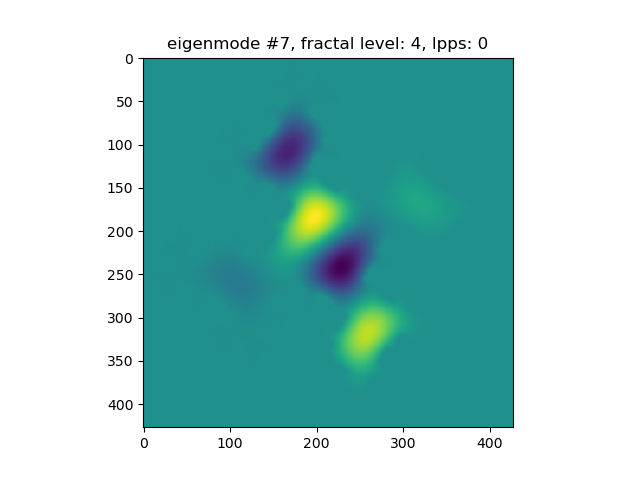
\includegraphics[width=\linewidth]{../figs/eigenmode_2d7.png}
    \end{subfigure}
    \begin{subfigure}{0.3\textwidth}
        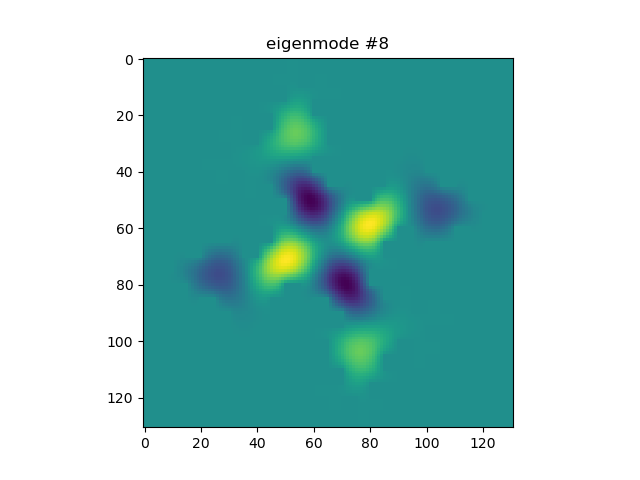
\includegraphics[width=\linewidth]{../figs/eigenmode_2d8.png}
    \end{subfigure}
    \begin{subfigure}{0.3\textwidth}
        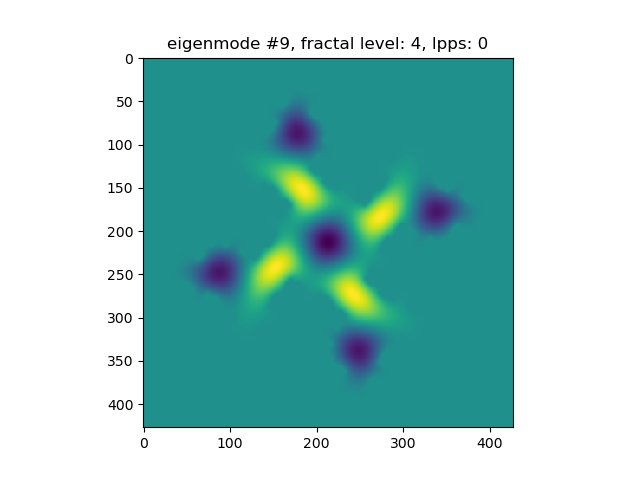
\includegraphics[width=\linewidth]{../figs/eigenmode_2d9.png}
    \end{subfigure}
    \begin{subfigure}{0.3\textwidth}
        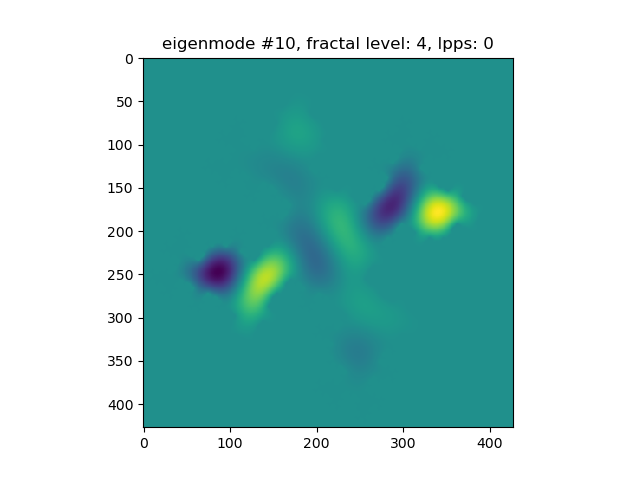
\includegraphics[width=\linewidth]{../figs/eigenmode_2d10.png}
    \end{subfigure}
    \caption{The 10 lowest eigenmodes, 2D plots.}
    \label{2dmodes}
\end{figure}

\end{document}

